\section{Implementering af DSP modul}\label{sec:implementering_dsp}
DSP modulet har til opgave at beregne koefficienter, beregne amplitude (til lcd'en), udføre det 
digitale filter på de samples der modtages mm.. På figur \ref{fig:dsp_flow_diag} illuteres data flow'et 
som kommunikerer med equalizer modulet.

\begin{figure}[h]
\centering
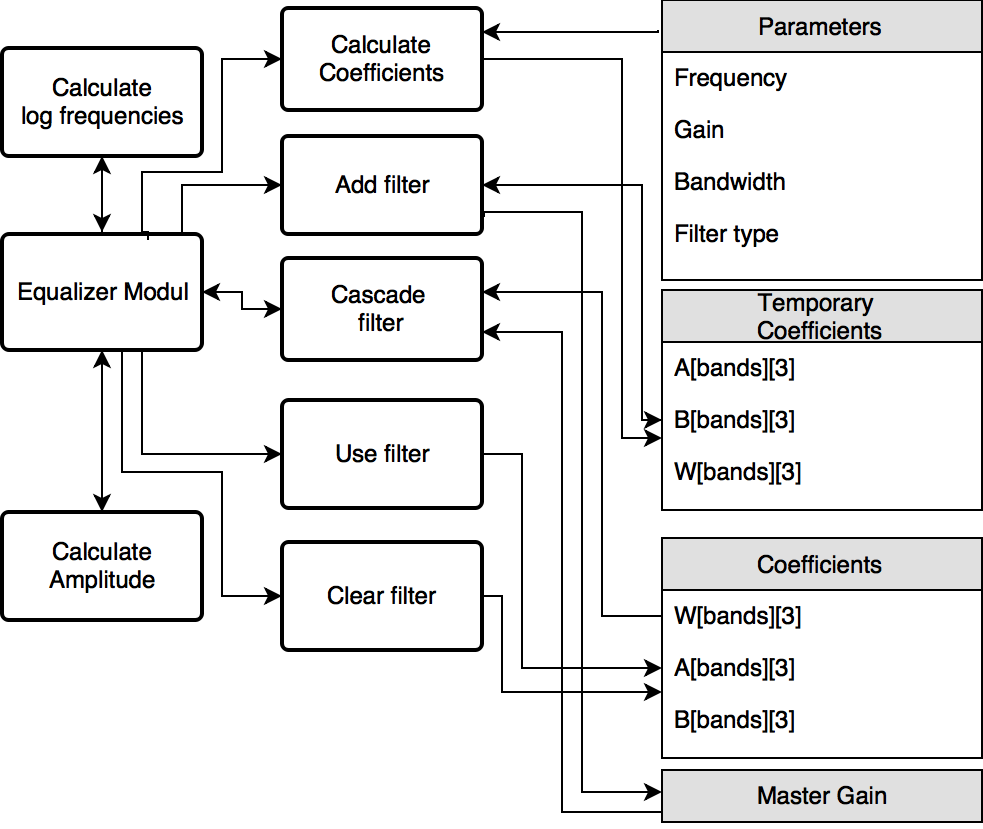
\includegraphics[scale = 0.3]{billeder/dsp_flowdiagram}
\caption{Flowdiagram af dsp modulet.}
\label{fig:dsp_flow_diag}
\end{figure}


active\_band holder styr på hvor mange bånd equalizer har.



Funktionaliteter:
\begin{itemize}[noitemsep,nolistsep]
\item Calculate Amplitude: modtager en frekvens og returnerer amplituden i $dB$.  \\
\item Calculate Coefficients: modtager parametre og beregner koefficienter. \\
\item Add filter: modtager koefficienter og overfører dem til temp bufferen. Inkrementerer active\_band.\\
\item Use filter: overfører koefficienterne fra temp bufferen til bufferen \\
\item Clear filter: nulstiller $W$  \\
\item Cascade filter: modtager et sample som skal filtreres, henter koefficienterne fra bufferen.
\end{itemize}